\documentclass[1p]{elsarticle_modified}
%\bibliographystyle{elsarticle-num}

%\usepackage[colorlinks]{hyperref}
%\usepackage{abbrmath_seonhwa} %\Abb, \Ascr, \Acal ,\Abf, \Afrak
\usepackage{amsfonts}
\usepackage{amssymb}
\usepackage{amsmath}
\usepackage{amsthm}
\usepackage{scalefnt}
\usepackage{amsbsy}
\usepackage{kotex}
\usepackage{caption}
\usepackage{subfig}
\usepackage{color}
\usepackage{graphicx}
\usepackage{xcolor} %% white, black, red, green, blue, cyan, magenta, yellow
\usepackage{float}
\usepackage{setspace}
\usepackage{hyperref}

\usepackage{tikz}
\usetikzlibrary{arrows}

\usepackage{multirow}
\usepackage{array} % fixed length table
\usepackage{hhline}

%%%%%%%%%%%%%%%%%%%%%
\makeatletter
\renewcommand*\env@matrix[1][\arraystretch]{%
	\edef\arraystretch{#1}%
	\hskip -\arraycolsep
	\let\@ifnextchar\new@ifnextchar
	\array{*\c@MaxMatrixCols c}}
\makeatother %https://tex.stackexchange.com/questions/14071/how-can-i-increase-the-line-spacing-in-a-matrix
%%%%%%%%%%%%%%%

\usepackage[normalem]{ulem}

\newcommand{\msout}[1]{\ifmmode\text{\sout{\ensuremath{#1}}}\else\sout{#1}\fi}
%SOURCE: \msout is \stkout macro in https://tex.stackexchange.com/questions/20609/strikeout-in-math-mode

\newcommand{\cancel}[1]{
	\ifmmode
	{\color{red}\msout{#1}}
	\else
	{\color{red}\sout{#1}}
	\fi
}

\newcommand{\add}[1]{
	{\color{blue}\uwave{#1}}
}

\newcommand{\replace}[2]{
	\ifmmode
	{\color{red}\msout{#1}}{\color{blue}\uwave{#2}}
	\else
	{\color{red}\sout{#1}}{\color{blue}\uwave{#2}}
	\fi
}

\newcommand{\Sol}{\mathcal{S}} %segment
\newcommand{\D}{D} %diagram
\newcommand{\A}{\mathcal{A}} %arc


%%%%%%%%%%%%%%%%%%%%%%%%%%%%%5 test

\def\sl{\operatorname{\textup{SL}}(2,\Cbb)}
\def\psl{\operatorname{\textup{PSL}}(2,\Cbb)}
\def\quan{\mkern 1mu \triangleright \mkern 1mu}

\theoremstyle{definition}
\newtheorem{thm}{Theorem}[section]
\newtheorem{prop}[thm]{Proposition}
\newtheorem{lem}[thm]{Lemma}
\newtheorem{ques}[thm]{Question}
\newtheorem{cor}[thm]{Corollary}
\newtheorem{defn}[thm]{Definition}
\newtheorem{exam}[thm]{Example}
\newtheorem{rmk}[thm]{Remark}
\newtheorem{alg}[thm]{Algorithm}

\newcommand{\I}{\sqrt{-1}}
\begin{document}

%\begin{frontmatter}
%
%\title{Boundary parabolic representations of knots up to 8 crossings}
%
%%% Group authors per affiliation:
%\author{Yunhi Cho} 
%\address{Department of Mathematics, University of Seoul, Seoul, Korea}
%\ead{yhcho@uos.ac.kr}
%
%
%\author{Seonhwa Kim} %\fnref{s_kim}}
%\address{Center for Geometry and Physics, Institute for Basic Science, Pohang, 37673, Korea}
%\ead{ryeona17@ibs.re.kr}
%
%\author{Hyuk Kim}
%\address{Department of Mathematical Sciences, Seoul National University, Seoul 08826, Korea}
%\ead{hyukkim@snu.ac.kr}
%
%\author{Seokbeom Yoon}
%\address{Department of Mathematical Sciences, Seoul National University, Seoul, 08826,  Korea}
%\ead{sbyoon15@snu.ac.kr}
%
%\begin{abstract}
%We find all boundary parabolic representation of knots up to 8 crossings.
%
%\end{abstract}
%\begin{keyword}
%    \MSC[2010] 57M25 
%\end{keyword}
%
%\end{frontmatter}

%\linenumbers
%\tableofcontents
%
\newcommand\colored[1]{\textcolor{white}{\rule[-0.35ex]{0.8em}{1.4ex}}\kern-0.8em\color{red} #1}%
%\newcommand\colored[1]{\textcolor{white}{ #1}\kern-2.17ex	\textcolor{white}{ #1}\kern-1.81ex	\textcolor{white}{ #1}\kern-2.15ex\color{red}#1	}

{\Large $\underline{12a_{0466}~(K12a_{0466})}$}

\setlength{\tabcolsep}{10pt}
\renewcommand{\arraystretch}{1.6}
\vspace{1cm}\begin{tabular}{m{100pt}>{\centering\arraybackslash}m{274pt}}
\multirow{5}{120pt}{
	\centering
	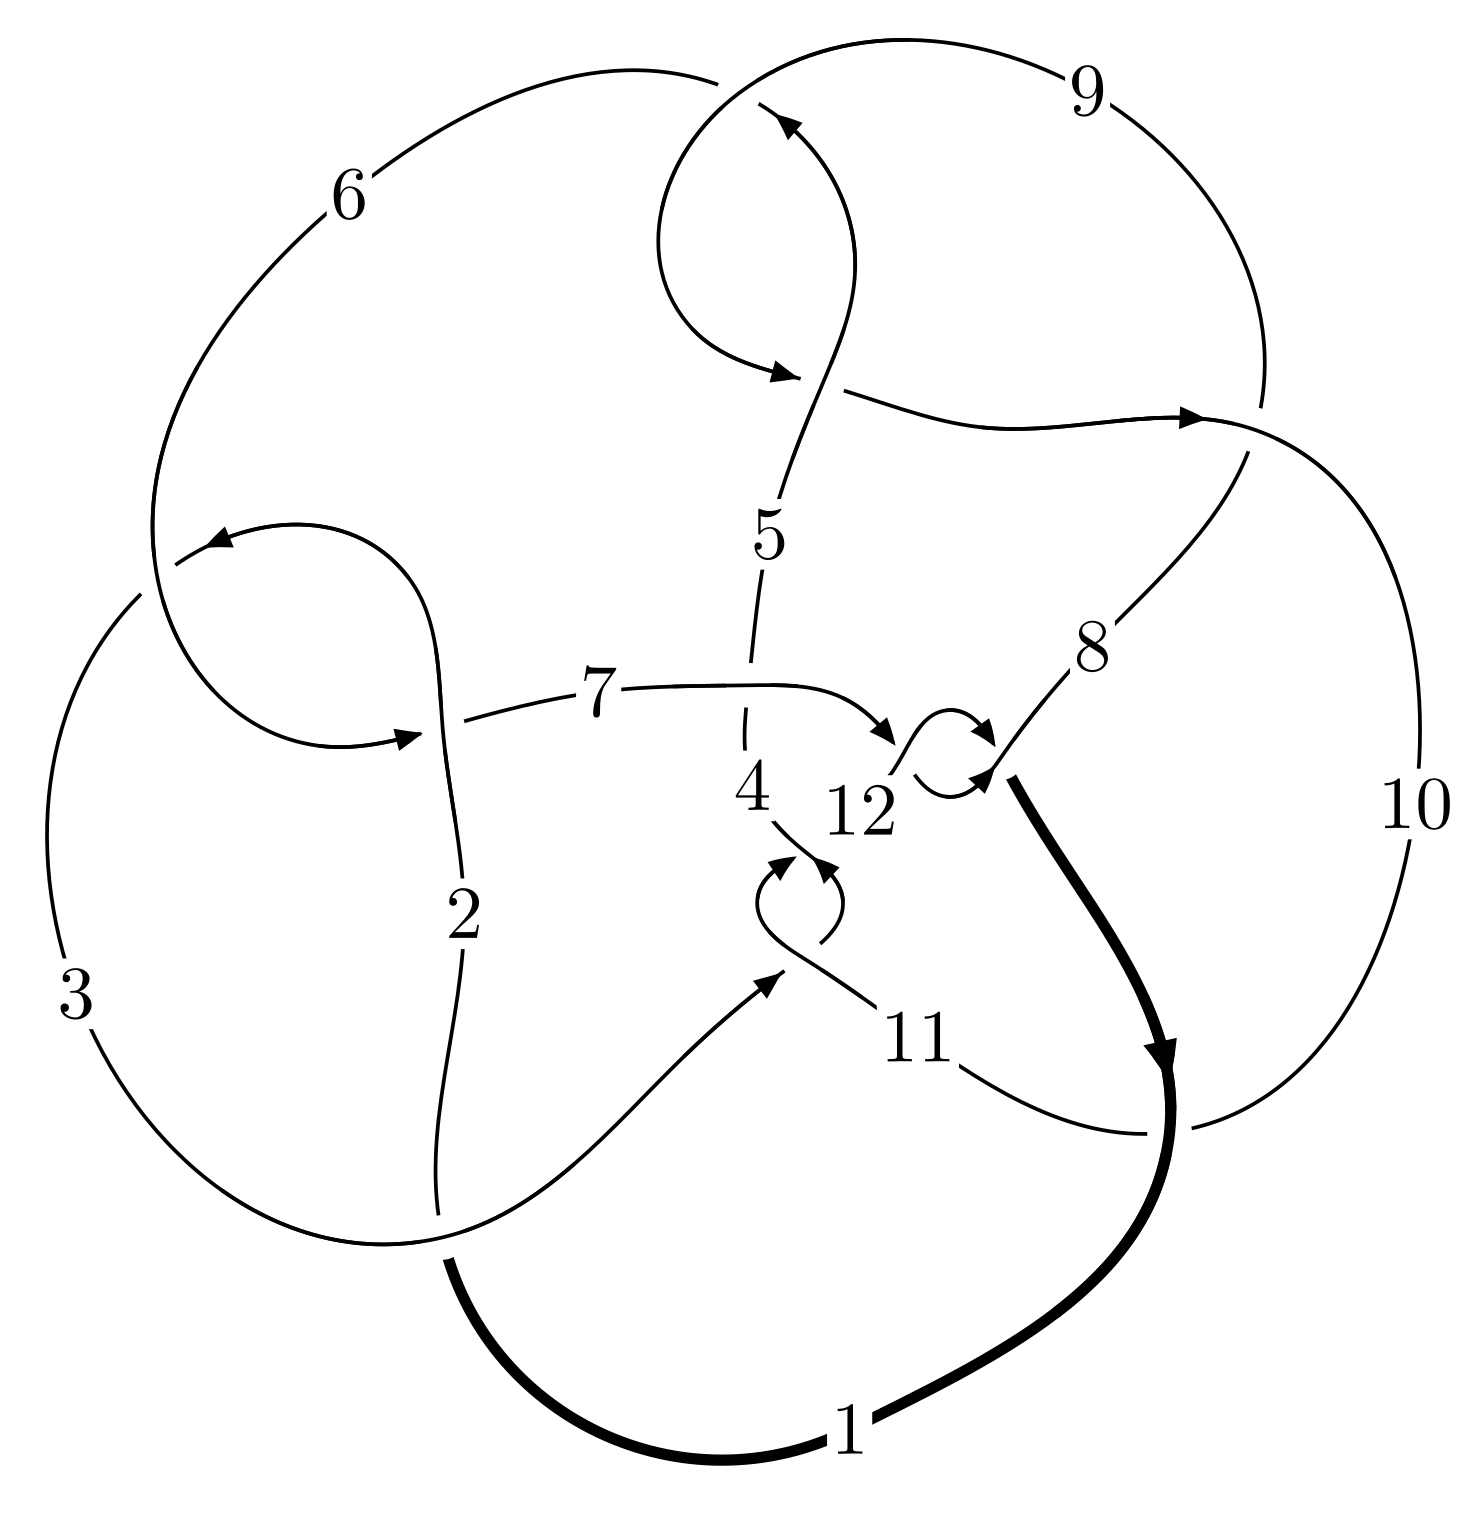
\includegraphics[width=112pt]{../../../GIT/diagram.site/Diagrams/png/1267_12a_0466.png}\\
\ \ \ A knot diagram\footnotemark}&
\allowdisplaybreaks
\textbf{Linearized knot diagam} \\
\cline{2-2}
 &
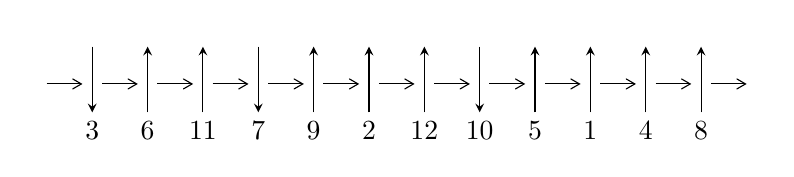
\begin{tikzpicture}[x=20pt, y=17pt]
	% nodes
	\node (C0) at (0, 0) {};
	\node (C1) at (1, 0) {};
	\node (C1U) at (1, +1) {};
	\node (C1D) at (1, -1) {3};

	\node (C2) at (2, 0) {};
	\node (C2U) at (2, +1) {};
	\node (C2D) at (2, -1) {6};

	\node (C3) at (3, 0) {};
	\node (C3U) at (3, +1) {};
	\node (C3D) at (3, -1) {11};

	\node (C4) at (4, 0) {};
	\node (C4U) at (4, +1) {};
	\node (C4D) at (4, -1) {7};

	\node (C5) at (5, 0) {};
	\node (C5U) at (5, +1) {};
	\node (C5D) at (5, -1) {9};

	\node (C6) at (6, 0) {};
	\node (C6U) at (6, +1) {};
	\node (C6D) at (6, -1) {2};

	\node (C7) at (7, 0) {};
	\node (C7U) at (7, +1) {};
	\node (C7D) at (7, -1) {12};

	\node (C8) at (8, 0) {};
	\node (C8U) at (8, +1) {};
	\node (C8D) at (8, -1) {10};

	\node (C9) at (9, 0) {};
	\node (C9U) at (9, +1) {};
	\node (C9D) at (9, -1) {5};

	\node (C10) at (10, 0) {};
	\node (C10U) at (10, +1) {};
	\node (C10D) at (10, -1) {1};

	\node (C11) at (11, 0) {};
	\node (C11U) at (11, +1) {};
	\node (C11D) at (11, -1) {4};

	\node (C12) at (12, 0) {};
	\node (C12U) at (12, +1) {};
	\node (C12D) at (12, -1) {8};
	\node (C13) at (13, 0) {};

	% arrows
	\draw[->,>={angle 60}]
	(C0) edge (C1) (C1) edge (C2) (C2) edge (C3) (C3) edge (C4) (C4) edge (C5) (C5) edge (C6) (C6) edge (C7) (C7) edge (C8) (C8) edge (C9) (C9) edge (C10) (C10) edge (C11) (C11) edge (C12) (C12) edge (C13) ;	\draw[->,>=stealth]
	(C1U) edge (C1D) (C2D) edge (C2U) (C3D) edge (C3U) (C4U) edge (C4D) (C5D) edge (C5U) (C6D) edge (C6U) (C7D) edge (C7U) (C8U) edge (C8D) (C9D) edge (C9U) (C10D) edge (C10U) (C11D) edge (C11U) (C12D) edge (C12U) ;
	\end{tikzpicture} \\
\hhline{~~} \\& 
\textbf{Solving Sequence} \\ \cline{2-2} 
 &
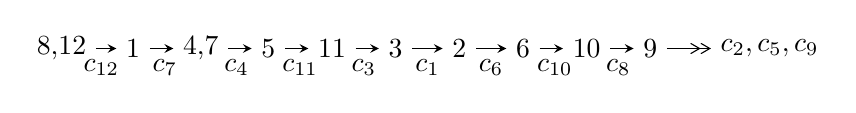
\begin{tikzpicture}[x=23pt, y=7pt]
	% node
	\node (A0) at (-1/8, 0) {8,12};
	\node (A1) at (1, 0) {1};
	\node (A2) at (33/16, 0) {4,7};
	\node (A3) at (25/8, 0) {5};
	\node (A4) at (33/8, 0) {11};
	\node (A5) at (41/8, 0) {3};
	\node (A6) at (49/8, 0) {2};
	\node (A7) at (57/8, 0) {6};
	\node (A8) at (65/8, 0) {10};
	\node (A9) at (73/8, 0) {9};
	\node (C1) at (1/2, -1) {$c_{12}$};
	\node (C2) at (3/2, -1) {$c_{7}$};
	\node (C3) at (21/8, -1) {$c_{4}$};
	\node (C4) at (29/8, -1) {$c_{11}$};
	\node (C5) at (37/8, -1) {$c_{3}$};
	\node (C6) at (45/8, -1) {$c_{1}$};
	\node (C7) at (53/8, -1) {$c_{6}$};
	\node (C8) at (61/8, -1) {$c_{10}$};
	\node (C9) at (69/8, -1) {$c_{8}$};
	\node (A10) at (11, 0) {$c_{2},c_{5},c_{9}$};

	% edge
	\draw[->,>=stealth]	
	(A0) edge (A1) (A1) edge (A2) (A2) edge (A3) (A3) edge (A4) (A4) edge (A5) (A5) edge (A6) (A6) edge (A7) (A7) edge (A8) (A8) edge (A9) ;
	\draw[->>,>={angle 60}]	
	(A9) edge (A10);
\end{tikzpicture} \\ 

\end{tabular} \\

\footnotetext{
The image of knot diagram is generated by the software ``\textbf{Draw programme}" developed by Andrew Bartholomew(\url{http://www.layer8.co.uk/maths/draw/index.htm\#Running-draw}), where we modified some parts for our purpose(\url{https://github.com/CATsTAILs/LinksPainter}).
}\phantom \\ \newline 
\centering \textbf{Ideals for irreducible components\footnotemark of $X_{\text{par}}$} 
 
\begin{align*}
I^u_{1}&=\langle 
b- u,\;3747 u^{13}-7659 u^{12}+\cdots+14581 a+18101,\\
\phantom{I^u_{1}}&\phantom{= \langle  }u^{14}-5 u^{12}+10 u^{10}+2 u^9-5 u^8-6 u^7-4 u^6+4 u^5+4 u^4+7 u^3-1\rangle \\
I^u_{2}&=\langle 
5.39240\times10^{368} u^{101}-7.26688\times10^{368} u^{100}+\cdots+4.52702\times10^{370} b-8.26613\times10^{371},\\
\phantom{I^u_{2}}&\phantom{= \langle  }-7.29228\times10^{372} u^{101}+2.80450\times10^{373} u^{100}+\cdots+1.94571\times10^{374} a-1.76617\times10^{376},\\
\phantom{I^u_{2}}&\phantom{= \langle  }u^{102}-3 u^{101}+\cdots+6720 u+1228\rangle \\
I^u_{3}&=\langle 
b-1,\;18 a^2-3 a u+24 a-2 u+7,\;u^2+2\rangle \\
I^u_{4}&=\langle 
54 a^3-27 a^2+58 b+153 a-25,\;27 a^4-18 a^3+57 a^2-18 a+19,\;u+1\rangle \\
I^u_{5}&=\langle 
b,\;a^2- a+1,\;u-1\rangle \\
\\
I^v_{1}&=\langle 
a,\;b+1,\;v^2- v+1\rangle \\
\end{align*}
\raggedright * 6 irreducible components of $\dim_{\mathbb{C}}=0$, with total 128 representations.\\
\footnotetext{All coefficients of polynomials are rational numbers. But the coefficients are sometimes approximated in decimal forms when there is not enough margin.}
\newpage
\renewcommand{\arraystretch}{1}
\centering \section*{I. $I^u_{1}= \langle b- u,\;3747 u^{13}-7659 u^{12}+\cdots+14581 a+18101,\;u^{14}-5 u^{12}+\cdots+7 u^3-1 \rangle$}
\flushleft \textbf{(i) Arc colorings}\\
\begin{tabular}{m{7pt} m{180pt} m{7pt} m{180pt} }
\flushright $a_{8}=$&$\begin{pmatrix}0\\u\end{pmatrix}$ \\
\flushright $a_{12}=$&$\begin{pmatrix}1\\0\end{pmatrix}$ \\
\flushright $a_{1}=$&$\begin{pmatrix}1\\- u^2\end{pmatrix}$ \\
\flushright $a_{4}=$&$\begin{pmatrix}-0.256978 u^{13}+0.525273 u^{12}+\cdots+1.54427 u-1.24141\\u\end{pmatrix}$ \\
\flushright $a_{7}=$&$\begin{pmatrix}- u\\u\end{pmatrix}$ \\
\flushright $a_{5}=$&$\begin{pmatrix}0.0739318 u^{13}+0.434950 u^{12}+\cdots+1.80125 u-1.76668\\-0.330910 u^{13}+0.0903230 u^{12}+\cdots+0.743022 u+0.525273\end{pmatrix}$ \\
\flushright $a_{11}=$&$\begin{pmatrix}0.525273 u^{13}-0.330910 u^{12}+\cdots-1.24141 u+0.743022\\u^2\end{pmatrix}$ \\
\flushright $a_{3}=$&$\begin{pmatrix}0.0739318 u^{13}+0.434950 u^{12}+\cdots+0.801248 u-1.76668\\- u^3+u\end{pmatrix}$ \\
\flushright $a_{2}=$&$\begin{pmatrix}0.355737 u^{13}-0.504561 u^{12}+\cdots-1.69659 u+1.25252\\0.149304 u^{13}+0.216035 u^{12}+\cdots+0.364858 u-0.645703\end{pmatrix}$ \\
\flushright $a_{6}=$&$\begin{pmatrix}u^2-1\\-0.434950 u^{13}+0.467115 u^{12}+\cdots+1.76668 u-0.0739318\end{pmatrix}$ \\
\flushright $a_{10}=$&$\begin{pmatrix}0.434950 u^{13}-0.467115 u^{12}+\cdots-1.76668 u+1.07393\\0.0202318 u^{13}-0.0423839 u^{12}+\cdots+0.0903230 u+0.136205\end{pmatrix}$ \\
\flushright $a_{9}=$&$\begin{pmatrix}1.15026 u^{13}-0.219875 u^{12}+\cdots-1.79357 u-0.720595\\-0.269392 u^{13}+0.0181058 u^{12}+\cdots+1.02105 u+0.155408\end{pmatrix}$\\&\end{tabular}
\flushleft \textbf{(ii) Obstruction class $= -1$}\\~\\
\flushleft \textbf{(iii) Cusp Shapes $= \frac{6748}{2083} u^{13}-\frac{6908}{14581} u^{12}+\cdots+\frac{3068}{2083} u+\frac{110818}{14581}$}\\~\\
\newpage\renewcommand{\arraystretch}{1}
\flushleft \textbf{(iv) u-Polynomials at the component}\newline \\
\begin{tabular}{m{50pt}|m{274pt}}
Crossings & \hspace{64pt}u-Polynomials at each crossing \\
\hline $$\begin{aligned}c_{1},c_{8}\end{aligned}$$&$\begin{aligned}
&u^{14}+6 u^{13}+\cdots-8 u+1
\end{aligned}$\\
\hline $$\begin{aligned}c_{2},c_{5},c_{6}\\c_{9}\end{aligned}$$&$\begin{aligned}
&u^{14}+3 u^{12}+6 u^{10}+7 u^8-2 u^7+6 u^6-4 u^5+6 u^4-5 u^3+4 u^2-4 u+1
\end{aligned}$\\
\hline $$\begin{aligned}c_{3},c_{7},c_{11}\\c_{12}\end{aligned}$$&$\begin{aligned}
&u^{14}-5 u^{12}+10 u^{10}+2 u^9-5 u^8-6 u^7-4 u^6+4 u^5+4 u^4+7 u^3-1
\end{aligned}$\\
\hline $$\begin{aligned}c_{4}\end{aligned}$$&$\begin{aligned}
&49(49 u^{14}-567 u^{13}+\cdots-6400 u+512)
\end{aligned}$\\
\hline $$\begin{aligned}c_{10}\end{aligned}$$&$\begin{aligned}
&49(49 u^{14}+567 u^{13}+\cdots-256 u-32)
\end{aligned}$\\
\hline
\end{tabular}\\~\\
\newpage\renewcommand{\arraystretch}{1}
\flushleft \textbf{(v) Riley Polynomials at the component}\newline \\
\begin{tabular}{m{50pt}|m{274pt}}
Crossings & \hspace{64pt}Riley Polynomials at each crossing \\
\hline $$\begin{aligned}c_{1},c_{8}\end{aligned}$$&$\begin{aligned}
&y^{14}+6 y^{13}+\cdots-88 y+1
\end{aligned}$\\
\hline $$\begin{aligned}c_{2},c_{5},c_{6}\\c_{9}\end{aligned}$$&$\begin{aligned}
&y^{14}+6 y^{13}+\cdots-8 y+1
\end{aligned}$\\
\hline $$\begin{aligned}c_{3},c_{7},c_{11}\\c_{12}\end{aligned}$$&$\begin{aligned}
&y^{14}-10 y^{13}+\cdots-8 y^2+1
\end{aligned}$\\
\hline $$\begin{aligned}c_{4}\end{aligned}$$&$\begin{aligned}
&2401(2401 y^{14}+13671 y^{13}+\cdots-8978432 y+262144)
\end{aligned}$\\
\hline $$\begin{aligned}c_{10}\end{aligned}$$&$\begin{aligned}
&2401(2401 y^{14}-27489 y^{13}+\cdots-15872 y+1024)
\end{aligned}$\\
\hline
\end{tabular}\\~\\
\newpage\flushleft \textbf{(vi) Complex Volumes and Cusp Shapes}
$$\begin{array}{c|c|c}  
\text{Solutions to }I^u_{1}& \I (\text{vol} + \sqrt{-1}CS) & \text{Cusp shape}\\
 \hline 
\begin{aligned}
u &= -0.516196 + 0.668974 I \\
a &= \phantom{-}1.017360 + 0.288726 I \\
b &= -0.516196 + 0.668974 I\end{aligned}
 & -5.02201 - 5.08838 I & -1.61799 + 8.05922 I \\ \hline\begin{aligned}
u &= -0.516196 - 0.668974 I \\
a &= \phantom{-}1.017360 - 0.288726 I \\
b &= -0.516196 - 0.668974 I\end{aligned}
 & -5.02201 + 5.08838 I & -1.61799 - 8.05922 I \\ \hline\begin{aligned}
u &= \phantom{-}0.049265 + 0.817919 I \\
a &= \phantom{-}0.729990 + 0.633371 I \\
b &= \phantom{-}0.049265 + 0.817919 I\end{aligned}
 & -0.60028 + 8.39490 I & \phantom{-}2.98961 - 7.37830 I \\ \hline\begin{aligned}
u &= \phantom{-}0.049265 - 0.817919 I \\
a &= \phantom{-}0.729990 - 0.633371 I \\
b &= \phantom{-}0.049265 - 0.817919 I\end{aligned}
 & -0.60028 - 8.39490 I & \phantom{-}2.98961 + 7.37830 I \\ \hline\begin{aligned}
u &= \phantom{-}1.187260 + 0.433713 I \\
a &= -1.66682 + 0.63904 I \\
b &= \phantom{-}1.187260 + 0.433713 I\end{aligned}
 & -0.83636 + 3.84412 I & \phantom{-}2.45895 - 3.50905 I \\ \hline\begin{aligned}
u &= \phantom{-}1.187260 - 0.433713 I \\
a &= -1.66682 - 0.63904 I \\
b &= \phantom{-}1.187260 - 0.433713 I\end{aligned}
 & -0.83636 - 3.84412 I & \phantom{-}2.45895 + 3.50905 I \\ \hline\begin{aligned}
u &= -1.33396\phantom{ +0.000000I} \\
a &= \phantom{-}2.15674\phantom{ +0.000000I} \\
b &= -1.33396\phantom{ +0.000000I}\end{aligned}
 & \phantom{-}6.74792\phantom{ +0.000000I} & \phantom{-}14.5770\phantom{ +0.000000I} \\ \hline\begin{aligned}
u &= -0.261143 + 0.528763 I \\
a &= -1.18448 + 0.94699 I \\
b &= -0.261143 + 0.528763 I\end{aligned}
 & \phantom{-}1.62602 + 1.81371 I & \phantom{-}5.85449 - 2.18660 I \\ \hline\begin{aligned}
u &= -0.261143 - 0.528763 I \\
a &= -1.18448 - 0.94699 I \\
b &= -0.261143 - 0.528763 I\end{aligned}
 & \phantom{-}1.62602 - 1.81371 I & \phantom{-}5.85449 + 2.18660 I \\ \hline\begin{aligned}
u &= \phantom{-}0.480208\phantom{ +0.000000I} \\
a &= -0.845526\phantom{ +0.000000I} \\
b &= \phantom{-}0.480208\phantom{ +0.000000I}\end{aligned}
 & \phantom{-}0.732652\phantom{ +0.000000I} & \phantom{-}13.8190\phantom{ +0.000000I}\\
 \hline 
 \end{array}$$\newpage$$\begin{array}{c|c|c}  
\text{Solutions to }I^u_{1}& \I (\text{vol} + \sqrt{-1}CS) & \text{Cusp shape}\\
 \hline 
\begin{aligned}
u &= \phantom{-}1.45636 + 0.53970 I \\
a &= -1.66668 + 0.71755 I \\
b &= \phantom{-}1.45636 + 0.53970 I\end{aligned}
 & \phantom{-}8.7153 + 19.0009 I & \phantom{-}9.38864 - 10.26527 I \\ \hline\begin{aligned}
u &= \phantom{-}1.45636 - 0.53970 I \\
a &= -1.66668 - 0.71755 I \\
b &= \phantom{-}1.45636 - 0.53970 I\end{aligned}
 & \phantom{-}8.7153 - 19.0009 I & \phantom{-}9.38864 + 10.26527 I \\ \hline\begin{aligned}
u &= -1.48868 + 0.46189 I \\
a &= \phantom{-}1.61503 + 0.60076 I \\
b &= -1.48868 + 0.46189 I\end{aligned}
 & \phantom{-}12.11620 - 6.67391 I & \phantom{-}13.58514 + 1.84206 I \\ \hline\begin{aligned}
u &= -1.48868 - 0.46189 I \\
a &= \phantom{-}1.61503 - 0.60076 I \\
b &= -1.48868 - 0.46189 I\end{aligned}
 & \phantom{-}12.11620 + 6.67391 I & \phantom{-}13.58514 - 1.84206 I\\
 \hline 
 \end{array}$$\newpage\newpage\renewcommand{\arraystretch}{1}
\centering \section*{II. $I^u_{2}= \langle 5.39\times10^{368} u^{101}-7.27\times10^{368} u^{100}+\cdots+4.53\times10^{370} b-8.27\times10^{371},\;-7.29\times10^{372} u^{101}+2.80\times10^{373} u^{100}+\cdots+1.95\times10^{374} a-1.77\times10^{376},\;u^{102}-3 u^{101}+\cdots+6720 u+1228 \rangle$}
\flushleft \textbf{(i) Arc colorings}\\
\begin{tabular}{m{7pt} m{180pt} m{7pt} m{180pt} }
\flushright $a_{8}=$&$\begin{pmatrix}0\\u\end{pmatrix}$ \\
\flushright $a_{12}=$&$\begin{pmatrix}1\\0\end{pmatrix}$ \\
\flushright $a_{1}=$&$\begin{pmatrix}1\\- u^2\end{pmatrix}$ \\
\flushright $a_{4}=$&$\begin{pmatrix}0.0374787 u^{101}-0.144138 u^{100}+\cdots+313.271 u+90.7725\\-0.0119116 u^{101}+0.0160523 u^{100}+\cdots+117.702 u+18.2596\end{pmatrix}$ \\
\flushright $a_{7}=$&$\begin{pmatrix}- u\\u\end{pmatrix}$ \\
\flushright $a_{5}=$&$\begin{pmatrix}0.0601079 u^{101}-0.156706 u^{100}+\cdots-0.634123 u+27.6729\\-0.0345408 u^{101}+0.0286206 u^{100}+\cdots+431.607 u+81.3592\end{pmatrix}$ \\
\flushright $a_{11}=$&$\begin{pmatrix}-0.0596673 u^{101}+0.232521 u^{100}+\cdots-592.389 u-163.559\\-0.0317617 u^{101}+0.0733669 u^{100}+\cdots+12.4678 u-8.62955\end{pmatrix}$ \\
\flushright $a_{3}=$&$\begin{pmatrix}-0.00617077 u^{101}+0.0554503 u^{100}+\cdots-356.870 u-88.3022\\-0.0245955 u^{101}+0.0557894 u^{100}+\cdots+26.7586 u-5.47531\end{pmatrix}$ \\
\flushright $a_{2}=$&$\begin{pmatrix}-0.00465371 u^{101}-0.0244415 u^{100}+\cdots+335.002 u+75.6856\\0.0104418 u^{101}-0.0279042 u^{100}+\cdots+9.19679 u+7.32337\end{pmatrix}$ \\
\flushright $a_{6}=$&$\begin{pmatrix}-0.00445873 u^{101}+0.0379717 u^{100}+\cdots-220.187 u-56.7212\\-0.0369380 u^{101}+0.0898244 u^{100}+\cdots+46.8346 u-7.57770\end{pmatrix}$ \\
\flushright $a_{10}=$&$\begin{pmatrix}-0.0393466 u^{101}+0.143102 u^{100}+\cdots-318.483 u-89.2086\\-0.0178019 u^{101}+0.0644717 u^{100}+\cdots-153.806 u-43.5741\end{pmatrix}$ \\
\flushright $a_{9}=$&$\begin{pmatrix}-0.0544767 u^{101}+0.177113 u^{100}+\cdots-336.426 u-101.063\\-0.0360286 u^{101}+0.136503 u^{100}+\cdots-317.173 u-93.1241\end{pmatrix}$\\&\end{tabular}
\flushleft \textbf{(ii) Obstruction class $= -1$}\\~\\
\flushleft \textbf{(iii) Cusp Shapes $= 0.0665059 u^{101}-0.191404 u^{100}+\cdots-267.385 u+0.0474288$}\\~\\
\newpage\renewcommand{\arraystretch}{1}
\flushleft \textbf{(iv) u-Polynomials at the component}\newline \\
\begin{tabular}{m{50pt}|m{274pt}}
Crossings & \hspace{64pt}u-Polynomials at each crossing \\
\hline $$\begin{aligned}c_{1},c_{8}\end{aligned}$$&$\begin{aligned}
&u^{102}+42 u^{101}+\cdots+107216 u+5776
\end{aligned}$\\
\hline $$\begin{aligned}c_{2},c_{5},c_{6}\\c_{9}\end{aligned}$$&$\begin{aligned}
&u^{102}-2 u^{101}+\cdots+172 u+76
\end{aligned}$\\
\hline $$\begin{aligned}c_{3},c_{7},c_{11}\\c_{12}\end{aligned}$$&$\begin{aligned}
&u^{102}-3 u^{101}+\cdots+6720 u+1228
\end{aligned}$\\
\hline $$\begin{aligned}c_{4}\end{aligned}$$&$\begin{aligned}
&49(7 u^{51}+68 u^{50}+\cdots-1074 u+167)^{2}
\end{aligned}$\\
\hline $$\begin{aligned}c_{10}\end{aligned}$$&$\begin{aligned}
&49(7 u^{51}-65 u^{50}+\cdots+4991 u-373)^{2}
\end{aligned}$\\
\hline
\end{tabular}\\~\\
\newpage\renewcommand{\arraystretch}{1}
\flushleft \textbf{(v) Riley Polynomials at the component}\newline \\
\begin{tabular}{m{50pt}|m{274pt}}
Crossings & \hspace{64pt}Riley Polynomials at each crossing \\
\hline $$\begin{aligned}c_{1},c_{8}\end{aligned}$$&$\begin{aligned}
&y^{102}+42 y^{101}+\cdots+456890624 y+33362176
\end{aligned}$\\
\hline $$\begin{aligned}c_{2},c_{5},c_{6}\\c_{9}\end{aligned}$$&$\begin{aligned}
&y^{102}+42 y^{101}+\cdots+107216 y+5776
\end{aligned}$\\
\hline $$\begin{aligned}c_{3},c_{7},c_{11}\\c_{12}\end{aligned}$$&$\begin{aligned}
&y^{102}-71 y^{101}+\cdots-636032 y+1507984
\end{aligned}$\\
\hline $$\begin{aligned}c_{4}\end{aligned}$$&$\begin{aligned}
&2401(49 y^{51}+738 y^{50}+\cdots-123072 y-27889)^{2}
\end{aligned}$\\
\hline $$\begin{aligned}c_{10}\end{aligned}$$&$\begin{aligned}
&2401(49 y^{51}-2279 y^{50}+\cdots+1.33762\times10^{7} y-139129)^{2}
\end{aligned}$\\
\hline
\end{tabular}\\~\\
\newpage\flushleft \textbf{(vi) Complex Volumes and Cusp Shapes}
$$\begin{array}{c|c|c}  
\text{Solutions to }I^u_{2}& \I (\text{vol} + \sqrt{-1}CS) & \text{Cusp shape}\\
 \hline 
\begin{aligned}
u &= -0.938800 + 0.219906 I \\
a &= -0.104097 - 0.814218 I \\
b &= \phantom{-}0.306890 + 1.203660 I\end{aligned}
 & -3.98676 + 1.42787 I & \phantom{-0.000000 } 0 \\ \hline\begin{aligned}
u &= -0.938800 - 0.219906 I \\
a &= -0.104097 + 0.814218 I \\
b &= \phantom{-}0.306890 - 1.203660 I\end{aligned}
 & -3.98676 - 1.42787 I & \phantom{-0.000000 } 0 \\ \hline\begin{aligned}
u &= -0.132342 + 0.952090 I \\
a &= \phantom{-}0.675049 + 0.192146 I \\
b &= -0.480609 + 0.312195 I\end{aligned}
 & -4.31975 + 1.46497 I & \phantom{-0.000000 } 0 \\ \hline\begin{aligned}
u &= -0.132342 - 0.952090 I \\
a &= \phantom{-}0.675049 - 0.192146 I \\
b &= -0.480609 - 0.312195 I\end{aligned}
 & -4.31975 - 1.46497 I & \phantom{-0.000000 } 0 \\ \hline\begin{aligned}
u &= \phantom{-}0.899835 + 0.223758 I \\
a &= \phantom{-}1.89347 - 0.47084 I \\
b &= \phantom{-}0.899835 - 0.223758 I\end{aligned}
 & \phantom{-}3.64125\phantom{ +0.000000I} & \phantom{-0.000000 } 0 \\ \hline\begin{aligned}
u &= \phantom{-}0.899835 - 0.223758 I \\
a &= \phantom{-}1.89347 + 0.47084 I \\
b &= \phantom{-}0.899835 + 0.223758 I\end{aligned}
 & \phantom{-}3.64125\phantom{ +0.000000I} & \phantom{-0.000000 } 0 \\ \hline\begin{aligned}
u &= -1.039410 + 0.270775 I \\
a &= -1.42959 + 1.12062 I \\
b &= -0.496445 + 0.034634 I\end{aligned}
 & \phantom{-}2.87536 - 0.22281 I & \phantom{-0.000000 } 0 \\ \hline\begin{aligned}
u &= -1.039410 - 0.270775 I \\
a &= -1.42959 - 1.12062 I \\
b &= -0.496445 - 0.034634 I\end{aligned}
 & \phantom{-}2.87536 + 0.22281 I & \phantom{-0.000000 } 0 \\ \hline\begin{aligned}
u &= \phantom{-}1.125680 + 0.169366 I \\
a &= \phantom{-}2.86751 - 0.62703 I \\
b &= -1.283310 + 0.005598 I\end{aligned}
 & \phantom{-}3.75261 + 3.46176 I & \phantom{-0.000000 } 0 \\ \hline\begin{aligned}
u &= \phantom{-}1.125680 - 0.169366 I \\
a &= \phantom{-}2.86751 + 0.62703 I \\
b &= -1.283310 - 0.005598 I\end{aligned}
 & \phantom{-}3.75261 - 3.46176 I & \phantom{-0.000000 } 0\\
 \hline 
 \end{array}$$\newpage$$\begin{array}{c|c|c}  
\text{Solutions to }I^u_{2}& \I (\text{vol} + \sqrt{-1}CS) & \text{Cusp shape}\\
 \hline 
\begin{aligned}
u &= \phantom{-}1.123400 + 0.263250 I \\
a &= -1.290530 - 0.397846 I \\
b &= -0.440373 + 0.187785 I\end{aligned}
 & \phantom{-}2.83235 - 4.49472 I & \phantom{-0.000000 } 0 \\ \hline\begin{aligned}
u &= \phantom{-}1.123400 - 0.263250 I \\
a &= -1.290530 + 0.397846 I \\
b &= -0.440373 - 0.187785 I\end{aligned}
 & \phantom{-}2.83235 + 4.49472 I & \phantom{-0.000000 } 0 \\ \hline\begin{aligned}
u &= -1.158280 + 0.038901 I \\
a &= -0.044900 - 1.082900 I \\
b &= \phantom{-}0.10892 + 1.76473 I\end{aligned}
 & -2.47417 - 2.36609 I & \phantom{-0.000000 } 0 \\ \hline\begin{aligned}
u &= -1.158280 - 0.038901 I \\
a &= -0.044900 + 1.082900 I \\
b &= \phantom{-}0.10892 - 1.76473 I\end{aligned}
 & -2.47417 + 2.36609 I & \phantom{-0.000000 } 0 \\ \hline\begin{aligned}
u &= \phantom{-}0.635991 + 0.544847 I \\
a &= \phantom{-}0.163228 + 0.980450 I \\
b &= \phantom{-}1.213660 + 0.118860 I\end{aligned}
 & \phantom{-}4.29974 - 0.52525 I & \phantom{-0.000000 } 0 \\ \hline\begin{aligned}
u &= \phantom{-}0.635991 - 0.544847 I \\
a &= \phantom{-}0.163228 - 0.980450 I \\
b &= \phantom{-}1.213660 - 0.118860 I\end{aligned}
 & \phantom{-}4.29974 + 0.52525 I & \phantom{-0.000000 } 0 \\ \hline\begin{aligned}
u &= \phantom{-}1.148780 + 0.231094 I \\
a &= -0.178896 + 0.316978 I \\
b &= \phantom{-}0.211521 - 0.622388 I\end{aligned}
 & \phantom{-}0.95763 + 1.31939 I & \phantom{-0.000000 } 0 \\ \hline\begin{aligned}
u &= \phantom{-}1.148780 - 0.231094 I \\
a &= -0.178896 - 0.316978 I \\
b &= \phantom{-}0.211521 + 0.622388 I\end{aligned}
 & \phantom{-}0.95763 - 1.31939 I & \phantom{-0.000000 } 0 \\ \hline\begin{aligned}
u &= \phantom{-}0.284402 + 1.150140 I \\
a &= \phantom{-}0.436714 - 0.359320 I \\
b &= -1.306890 - 0.351758 I\end{aligned}
 & \phantom{-}5.05561 + 7.21324 I & \phantom{-0.000000 } 0 \\ \hline\begin{aligned}
u &= \phantom{-}0.284402 - 1.150140 I \\
a &= \phantom{-}0.436714 + 0.359320 I \\
b &= -1.306890 + 0.351758 I\end{aligned}
 & \phantom{-}5.05561 - 7.21324 I & \phantom{-0.000000 } 0\\
 \hline 
 \end{array}$$\newpage$$\begin{array}{c|c|c}  
\text{Solutions to }I^u_{2}& \I (\text{vol} + \sqrt{-1}CS) & \text{Cusp shape}\\
 \hline 
\begin{aligned}
u &= \phantom{-}1.180890 + 0.101925 I \\
a &= -0.329287 + 0.402844 I \\
b &= \phantom{-}0.070577 - 0.397364 I\end{aligned}
 & \phantom{-}1.03755 + 1.42394 I & \phantom{-0.000000 } 0 \\ \hline\begin{aligned}
u &= \phantom{-}1.180890 - 0.101925 I \\
a &= -0.329287 - 0.402844 I \\
b &= \phantom{-}0.070577 + 0.397364 I\end{aligned}
 & \phantom{-}1.03755 - 1.42394 I & \phantom{-0.000000 } 0 \\ \hline\begin{aligned}
u &= -0.630547 + 0.473331 I \\
a &= -0.771433 - 0.171537 I \\
b &= \phantom{-}0.202395 - 0.600140 I\end{aligned}
 & -1.85835 - 1.85518 I & \phantom{-}2.88110 + 4.86946 I \\ \hline\begin{aligned}
u &= -0.630547 - 0.473331 I \\
a &= -0.771433 + 0.171537 I \\
b &= \phantom{-}0.202395 + 0.600140 I\end{aligned}
 & -1.85835 + 1.85518 I & \phantom{-}2.88110 - 4.86946 I \\ \hline\begin{aligned}
u &= \phantom{-}1.213660 + 0.118860 I \\
a &= -0.294299 + 0.615882 I \\
b &= \phantom{-}0.635991 + 0.544847 I\end{aligned}
 & \phantom{-}4.29974 - 0.52525 I & \phantom{-0.000000 } 0 \\ \hline\begin{aligned}
u &= \phantom{-}1.213660 - 0.118860 I \\
a &= -0.294299 - 0.615882 I \\
b &= \phantom{-}0.635991 - 0.544847 I\end{aligned}
 & \phantom{-}4.29974 + 0.52525 I & \phantom{-0.000000 } 0 \\ \hline\begin{aligned}
u &= -1.198720 + 0.266772 I \\
a &= -0.224557 - 0.808357 I \\
b &= \phantom{-}0.554100 - 0.529784 I\end{aligned}
 & \phantom{-}4.19644 - 4.78402 I & \phantom{-0.000000 } 0 \\ \hline\begin{aligned}
u &= -1.198720 - 0.266772 I \\
a &= -0.224557 + 0.808357 I \\
b &= \phantom{-}0.554100 + 0.529784 I\end{aligned}
 & \phantom{-}4.19644 + 4.78402 I & \phantom{-0.000000 } 0 \\ \hline\begin{aligned}
u &= \phantom{-}0.042252 + 0.768572 I \\
a &= \phantom{-}0.259981 - 0.234911 I \\
b &= -1.243120 + 0.401275 I\end{aligned}
 & -0.75830 - 6.15523 I & \phantom{-}2.54266 + 5.39268 I \\ \hline\begin{aligned}
u &= \phantom{-}0.042252 - 0.768572 I \\
a &= \phantom{-}0.259981 + 0.234911 I \\
b &= -1.243120 - 0.401275 I\end{aligned}
 & -0.75830 + 6.15523 I & \phantom{-}2.54266 - 5.39268 I\\
 \hline 
 \end{array}$$\newpage$$\begin{array}{c|c|c}  
\text{Solutions to }I^u_{2}& \I (\text{vol} + \sqrt{-1}CS) & \text{Cusp shape}\\
 \hline 
\begin{aligned}
u &= \phantom{-}0.554100 + 0.529784 I \\
a &= -0.362391 - 1.294170 I \\
b &= -1.198720 - 0.266772 I\end{aligned}
 & \phantom{-}4.19644 + 4.78402 I & \phantom{-}10.46471 - 6.58648 I \\ \hline\begin{aligned}
u &= \phantom{-}0.554100 - 0.529784 I \\
a &= -0.362391 + 1.294170 I \\
b &= -1.198720 + 0.266772 I\end{aligned}
 & \phantom{-}4.19644 - 4.78402 I & \phantom{-}10.46471 + 6.58648 I \\ \hline\begin{aligned}
u &= \phantom{-}0.306890 + 1.203660 I \\
a &= \phantom{-}0.633484 - 0.068432 I \\
b &= -0.938800 + 0.219906 I\end{aligned}
 & -3.98676 + 1.42787 I & \phantom{-0.000000 } 0 \\ \hline\begin{aligned}
u &= \phantom{-}0.306890 - 1.203660 I \\
a &= \phantom{-}0.633484 + 0.068432 I \\
b &= -0.938800 - 0.219906 I\end{aligned}
 & -3.98676 - 1.42787 I & \phantom{-0.000000 } 0 \\ \hline\begin{aligned}
u &= \phantom{-}0.028710 + 0.734651 I \\
a &= -0.946199 - 0.618995 I \\
b &= -0.209148 - 0.578349 I\end{aligned}
 & \phantom{-}0.87132 + 3.18706 I & \phantom{-}5.01381 - 3.27800 I \\ \hline\begin{aligned}
u &= \phantom{-}0.028710 - 0.734651 I \\
a &= -0.946199 + 0.618995 I \\
b &= -0.209148 + 0.578349 I\end{aligned}
 & \phantom{-}0.87132 - 3.18706 I & \phantom{-}5.01381 + 3.27800 I \\ \hline\begin{aligned}
u &= -0.721694 + 0.102104 I \\
a &= -0.322451 - 1.362520 I \\
b &= \phantom{-}0.021380 - 0.371251 I\end{aligned}
 & \phantom{-}0.94758 - 2.34060 I & \phantom{-}1.25710 + 5.53583 I \\ \hline\begin{aligned}
u &= -0.721694 - 0.102104 I \\
a &= -0.322451 + 1.362520 I \\
b &= \phantom{-}0.021380 + 0.371251 I\end{aligned}
 & \phantom{-}0.94758 + 2.34060 I & \phantom{-}1.25710 - 5.53583 I \\ \hline\begin{aligned}
u &= -0.132750 + 1.267920 I \\
a &= \phantom{-}0.533990 + 0.282704 I \\
b &= -1.318190 + 0.376845 I\end{aligned}
 & \phantom{-}3.68801 - 12.72800 I & \phantom{-0.000000 } 0 \\ \hline\begin{aligned}
u &= -0.132750 - 1.267920 I \\
a &= \phantom{-}0.533990 - 0.282704 I \\
b &= -1.318190 - 0.376845 I\end{aligned}
 & \phantom{-}3.68801 + 12.72800 I & \phantom{-0.000000 } 0\\
 \hline 
 \end{array}$$\newpage$$\begin{array}{c|c|c}  
\text{Solutions to }I^u_{2}& \I (\text{vol} + \sqrt{-1}CS) & \text{Cusp shape}\\
 \hline 
\begin{aligned}
u &= -1.283310 + 0.005598 I \\
a &= -2.59874 + 0.16023 I \\
b &= \phantom{-}1.125680 + 0.169366 I\end{aligned}
 & \phantom{-}3.75261 + 3.46176 I & \phantom{-0.000000 } 0 \\ \hline\begin{aligned}
u &= -1.283310 - 0.005598 I \\
a &= -2.59874 - 0.16023 I \\
b &= \phantom{-}1.125680 - 0.169366 I\end{aligned}
 & \phantom{-}3.75261 - 3.46176 I & \phantom{-0.000000 } 0 \\ \hline\begin{aligned}
u &= \phantom{-}1.255770 + 0.318257 I \\
a &= \phantom{-}1.98536 - 0.52012 I \\
b &= -1.56842 - 0.37132 I\end{aligned}
 & \phantom{-}4.44605 + 4.92843 I & \phantom{-0.000000 } 0 \\ \hline\begin{aligned}
u &= \phantom{-}1.255770 - 0.318257 I \\
a &= \phantom{-}1.98536 + 0.52012 I \\
b &= -1.56842 + 0.37132 I\end{aligned}
 & \phantom{-}4.44605 - 4.92843 I & \phantom{-0.000000 } 0 \\ \hline\begin{aligned}
u &= -1.243120 + 0.401275 I \\
a &= -0.094878 - 0.183378 I \\
b &= \phantom{-}0.042252 + 0.768572 I\end{aligned}
 & -0.75830 - 6.15523 I & \phantom{-0.000000 } 0 \\ \hline\begin{aligned}
u &= -1.243120 - 0.401275 I \\
a &= -0.094878 + 0.183378 I \\
b &= \phantom{-}0.042252 - 0.768572 I\end{aligned}
 & -0.75830 + 6.15523 I & \phantom{-0.000000 } 0 \\ \hline\begin{aligned}
u &= \phantom{-}0.294469 + 1.272850 I \\
a &= -0.491997 + 0.240143 I \\
b &= \phantom{-}1.315060 + 0.204346 I\end{aligned}
 & \phantom{-}6.39603 + 0.76029 I & \phantom{-0.000000 } 0 \\ \hline\begin{aligned}
u &= \phantom{-}0.294469 - 1.272850 I \\
a &= -0.491997 - 0.240143 I \\
b &= \phantom{-}1.315060 - 0.204346 I\end{aligned}
 & \phantom{-}6.39603 - 0.76029 I & \phantom{-0.000000 } 0 \\ \hline\begin{aligned}
u &= \phantom{-}1.279400 + 0.354549 I \\
a &= -1.92627 + 0.47196 I \\
b &= \phantom{-}1.57701 + 0.54463 I\end{aligned}
 & \phantom{-}3.13819 + 10.25710 I & \phantom{-0.000000 } 0 \\ \hline\begin{aligned}
u &= \phantom{-}1.279400 - 0.354549 I \\
a &= -1.92627 - 0.47196 I \\
b &= \phantom{-}1.57701 - 0.54463 I\end{aligned}
 & \phantom{-}3.13819 - 10.25710 I & \phantom{-0.000000 } 0\\
 \hline 
 \end{array}$$\newpage$$\begin{array}{c|c|c}  
\text{Solutions to }I^u_{2}& \I (\text{vol} + \sqrt{-1}CS) & \text{Cusp shape}\\
 \hline 
\begin{aligned}
u &= \phantom{-}1.315060 + 0.204346 I \\
a &= -0.398620 - 0.360491 I \\
b &= \phantom{-}0.294469 + 1.272850 I\end{aligned}
 & \phantom{-}6.39603 + 0.76029 I & \phantom{-0.000000 } 0 \\ \hline\begin{aligned}
u &= \phantom{-}1.315060 - 0.204346 I \\
a &= -0.398620 + 0.360491 I \\
b &= \phantom{-}0.294469 - 1.272850 I\end{aligned}
 & \phantom{-}6.39603 - 0.76029 I & \phantom{-0.000000 } 0 \\ \hline\begin{aligned}
u &= \phantom{-}1.333590 + 0.062848 I \\
a &= \phantom{-}1.70068 - 0.12225 I \\
b &= -1.62808 + 0.65945 I\end{aligned}
 & \phantom{-}8.12140 + 5.35202 I & \phantom{-0.000000 } 0 \\ \hline\begin{aligned}
u &= \phantom{-}1.333590 - 0.062848 I \\
a &= \phantom{-}1.70068 + 0.12225 I \\
b &= -1.62808 - 0.65945 I\end{aligned}
 & \phantom{-}8.12140 - 5.35202 I & \phantom{-0.000000 } 0 \\ \hline\begin{aligned}
u &= \phantom{-}1.335810 + 0.021201 I \\
a &= -1.52156 + 0.07833 I \\
b &= \phantom{-}1.48991 - 0.81435 I\end{aligned}
 & \phantom{-}8.28003 - 0.08726 I & \phantom{-0.000000 } 0 \\ \hline\begin{aligned}
u &= \phantom{-}1.335810 - 0.021201 I \\
a &= -1.52156 - 0.07833 I \\
b &= \phantom{-}1.48991 + 0.81435 I\end{aligned}
 & \phantom{-}8.28003 + 0.08726 I & \phantom{-0.000000 } 0 \\ \hline\begin{aligned}
u &= \phantom{-}1.319500 + 0.242954 I \\
a &= \phantom{-}0.302778 + 0.490529 I \\
b &= -0.081953 - 1.362050 I\end{aligned}
 & \phantom{-}5.54688 + 6.19194 I & \phantom{-0.000000 } 0 \\ \hline\begin{aligned}
u &= \phantom{-}1.319500 - 0.242954 I \\
a &= \phantom{-}0.302778 - 0.490529 I \\
b &= -0.081953 + 1.362050 I\end{aligned}
 & \phantom{-}5.54688 - 6.19194 I & \phantom{-0.000000 } 0 \\ \hline\begin{aligned}
u &= \phantom{-}0.211521 + 0.622388 I \\
a &= -0.601398 + 0.243507 I \\
b &= \phantom{-}1.148780 - 0.231094 I\end{aligned}
 & \phantom{-}0.95763 - 1.31939 I & \phantom{-}5.50400 - 0.11930 I \\ \hline\begin{aligned}
u &= \phantom{-}0.211521 - 0.622388 I \\
a &= -0.601398 - 0.243507 I \\
b &= \phantom{-}1.148780 + 0.231094 I\end{aligned}
 & \phantom{-}0.95763 + 1.31939 I & \phantom{-}5.50400 + 0.11930 I\\
 \hline 
 \end{array}$$\newpage$$\begin{array}{c|c|c}  
\text{Solutions to }I^u_{2}& \I (\text{vol} + \sqrt{-1}CS) & \text{Cusp shape}\\
 \hline 
\begin{aligned}
u &= -1.306890 + 0.351758 I \\
a &= -0.460310 + 0.182244 I \\
b &= \phantom{-}0.284402 - 1.150140 I\end{aligned}
 & \phantom{-}5.05561 - 7.21324 I & \phantom{-0.000000 } 0 \\ \hline\begin{aligned}
u &= -1.306890 - 0.351758 I \\
a &= -0.460310 - 0.182244 I \\
b &= \phantom{-}0.284402 + 1.150140 I\end{aligned}
 & \phantom{-}5.05561 + 7.21324 I & \phantom{-0.000000 } 0 \\ \hline\begin{aligned}
u &= -0.081953 + 1.362050 I \\
a &= -0.539640 - 0.173352 I \\
b &= \phantom{-}1.319500 - 0.242954 I\end{aligned}
 & \phantom{-}5.54688 - 6.19194 I & \phantom{-0.000000 } 0 \\ \hline\begin{aligned}
u &= -0.081953 - 1.362050 I \\
a &= -0.539640 + 0.173352 I \\
b &= \phantom{-}1.319500 + 0.242954 I\end{aligned}
 & \phantom{-}5.54688 + 6.19194 I & \phantom{-0.000000 } 0 \\ \hline\begin{aligned}
u &= \phantom{-}0.202395 + 0.600140 I \\
a &= \phantom{-}0.670871 - 0.719561 I \\
b &= -0.630547 - 0.473331 I\end{aligned}
 & -1.85835 + 1.85518 I & \phantom{-}2.88110 - 4.86946 I \\ \hline\begin{aligned}
u &= \phantom{-}0.202395 - 0.600140 I \\
a &= \phantom{-}0.670871 + 0.719561 I \\
b &= -0.630547 + 0.473331 I\end{aligned}
 & -1.85835 - 1.85518 I & \phantom{-}2.88110 + 4.86946 I \\ \hline\begin{aligned}
u &= -1.318190 + 0.376845 I \\
a &= \phantom{-}0.429309 - 0.362425 I \\
b &= -0.132750 + 1.267920 I\end{aligned}
 & \phantom{-}3.68801 - 12.72800 I & \phantom{-0.000000 } 0 \\ \hline\begin{aligned}
u &= -1.318190 - 0.376845 I \\
a &= \phantom{-}0.429309 + 0.362425 I \\
b &= -0.132750 - 1.267920 I\end{aligned}
 & \phantom{-}3.68801 + 12.72800 I & \phantom{-0.000000 } 0 \\ \hline\begin{aligned}
u &= -0.209148 + 0.578349 I \\
a &= \phantom{-}0.853649 - 1.048020 I \\
b &= \phantom{-}0.028710 - 0.734651 I\end{aligned}
 & \phantom{-}0.87132 - 3.18706 I & \phantom{-}5.01381 + 3.27800 I \\ \hline\begin{aligned}
u &= -0.209148 - 0.578349 I \\
a &= \phantom{-}0.853649 + 1.048020 I \\
b &= \phantom{-}0.028710 + 0.734651 I\end{aligned}
 & \phantom{-}0.87132 + 3.18706 I & \phantom{-}5.01381 - 3.27800 I\\
 \hline 
 \end{array}$$\newpage$$\begin{array}{c|c|c}  
\text{Solutions to }I^u_{2}& \I (\text{vol} + \sqrt{-1}CS) & \text{Cusp shape}\\
 \hline 
\begin{aligned}
u &= -1.389870 + 0.127948 I \\
a &= -1.64619 - 0.16333 I \\
b &= \phantom{-}1.53449 - 0.70295 I\end{aligned}
 & \phantom{-}10.26190 - 6.79269 I & \phantom{-0.000000 } 0 \\ \hline\begin{aligned}
u &= -1.389870 - 0.127948 I \\
a &= -1.64619 + 0.16333 I \\
b &= \phantom{-}1.53449 + 0.70295 I\end{aligned}
 & \phantom{-}10.26190 + 6.79269 I & \phantom{-0.000000 } 0 \\ \hline\begin{aligned}
u &= -1.393480 + 0.095069 I \\
a &= \phantom{-}1.75498 + 0.14814 I \\
b &= -1.61445 + 0.53714 I\end{aligned}
 & \phantom{-}10.66800 - 1.12994 I & \phantom{-0.000000 } 0 \\ \hline\begin{aligned}
u &= -1.393480 - 0.095069 I \\
a &= \phantom{-}1.75498 - 0.14814 I \\
b &= -1.61445 - 0.53714 I\end{aligned}
 & \phantom{-}10.66800 + 1.12994 I & \phantom{-0.000000 } 0 \\ \hline\begin{aligned}
u &= -0.480609 + 0.312195 I \\
a &= \phantom{-}0.985140 - 0.644437 I \\
b &= -0.132342 + 0.952090 I\end{aligned}
 & -4.31975 + 1.46497 I & -2.47124 - 1.07580 I \\ \hline\begin{aligned}
u &= -0.480609 - 0.312195 I \\
a &= \phantom{-}0.985140 + 0.644437 I \\
b &= -0.132342 - 0.952090 I\end{aligned}
 & -4.31975 - 1.46497 I & -2.47124 + 1.07580 I \\ \hline\begin{aligned}
u &= -0.496445 + 0.034634 I \\
a &= -2.58741 + 2.94549 I \\
b &= -1.039410 + 0.270775 I\end{aligned}
 & \phantom{-}2.87536 - 0.22281 I & \phantom{-}6.45523 + 2.31553 I \\ \hline\begin{aligned}
u &= -0.496445 - 0.034634 I \\
a &= -2.58741 - 2.94549 I \\
b &= -1.039410 - 0.270775 I\end{aligned}
 & \phantom{-}2.87536 + 0.22281 I & \phantom{-}6.45523 - 2.31553 I \\ \hline\begin{aligned}
u &= -0.440373 + 0.187785 I \\
a &= \phantom{-}1.93985 + 2.61358 I \\
b &= \phantom{-}1.123400 + 0.263250 I\end{aligned}
 & \phantom{-}2.83235 - 4.49472 I & \phantom{-}6.56893 + 6.15189 I \\ \hline\begin{aligned}
u &= -0.440373 - 0.187785 I \\
a &= \phantom{-}1.93985 - 2.61358 I \\
b &= \phantom{-}1.123400 - 0.263250 I\end{aligned}
 & \phantom{-}2.83235 + 4.49472 I & \phantom{-}6.56893 - 6.15189 I\\
 \hline 
 \end{array}$$\newpage$$\begin{array}{c|c|c}  
\text{Solutions to }I^u_{2}& \I (\text{vol} + \sqrt{-1}CS) & \text{Cusp shape}\\
 \hline 
\begin{aligned}
u &= -1.46278 + 0.45766 I \\
a &= -1.66720 - 0.61988 I \\
b &= \phantom{-}1.47529 - 0.56121 I\end{aligned}
 & \phantom{-}10.5630 - 12.8142 I & \phantom{-0.000000 } 0 \\ \hline\begin{aligned}
u &= -1.46278 - 0.45766 I \\
a &= -1.66720 + 0.61988 I \\
b &= \phantom{-}1.47529 + 0.56121 I\end{aligned}
 & \phantom{-}10.5630 + 12.8142 I & \phantom{-0.000000 } 0 \\ \hline\begin{aligned}
u &= \phantom{-}1.47529 + 0.56121 I \\
a &= \phantom{-}1.57971 - 0.69835 I \\
b &= -1.46278 - 0.45766 I\end{aligned}
 & \phantom{-}10.5630 + 12.8142 I & \phantom{-0.000000 } 0 \\ \hline\begin{aligned}
u &= \phantom{-}1.47529 - 0.56121 I \\
a &= \phantom{-}1.57971 + 0.69835 I \\
b &= -1.46278 + 0.45766 I\end{aligned}
 & \phantom{-}10.5630 - 12.8142 I & \phantom{-0.000000 } 0 \\ \hline\begin{aligned}
u &= \phantom{-}0.070577 + 0.397364 I \\
a &= -1.26496 + 0.85723 I \\
b &= \phantom{-}1.180890 - 0.101925 I\end{aligned}
 & \phantom{-}1.03755 - 1.42394 I & \phantom{-}2.53124 - 0.77932 I \\ \hline\begin{aligned}
u &= \phantom{-}0.070577 - 0.397364 I \\
a &= -1.26496 - 0.85723 I \\
b &= \phantom{-}1.180890 + 0.101925 I\end{aligned}
 & \phantom{-}1.03755 + 1.42394 I & \phantom{-}2.53124 + 0.77932 I \\ \hline\begin{aligned}
u &= -1.56842 + 0.37132 I \\
a &= -1.60212 - 0.39288 I \\
b &= \phantom{-}1.255770 - 0.318257 I\end{aligned}
 & \phantom{-}4.44605 - 4.92843 I & \phantom{-0.000000 } 0 \\ \hline\begin{aligned}
u &= -1.56842 - 0.37132 I \\
a &= -1.60212 + 0.39288 I \\
b &= \phantom{-}1.255770 + 0.318257 I\end{aligned}
 & \phantom{-}4.44605 + 4.92843 I & \phantom{-0.000000 } 0 \\ \hline\begin{aligned}
u &= \phantom{-}0.021380 + 0.371251 I \\
a &= -2.49403 - 1.14518 I \\
b &= -0.721694 - 0.102104 I\end{aligned}
 & \phantom{-}0.94758 + 2.34060 I & \phantom{-}1.25710 - 5.53583 I \\ \hline\begin{aligned}
u &= \phantom{-}0.021380 - 0.371251 I \\
a &= -2.49403 + 1.14518 I \\
b &= -0.721694 + 0.102104 I\end{aligned}
 & \phantom{-}0.94758 - 2.34060 I & \phantom{-}1.25710 + 5.53583 I\\
 \hline 
 \end{array}$$\newpage$$\begin{array}{c|c|c}  
\text{Solutions to }I^u_{2}& \I (\text{vol} + \sqrt{-1}CS) & \text{Cusp shape}\\
 \hline 
\begin{aligned}
u &= \phantom{-}1.57701 + 0.54463 I \\
a &= -1.50651 + 0.47010 I \\
b &= \phantom{-}1.279400 + 0.354549 I\end{aligned}
 & \phantom{-}3.13819 + 10.25710 I & \phantom{-0.000000 } 0 \\ \hline\begin{aligned}
u &= \phantom{-}1.57701 - 0.54463 I \\
a &= -1.50651 - 0.47010 I \\
b &= \phantom{-}1.279400 - 0.354549 I\end{aligned}
 & \phantom{-}3.13819 - 10.25710 I & \phantom{-0.000000 } 0 \\ \hline\begin{aligned}
u &= \phantom{-}1.53449 + 0.70295 I \\
a &= \phantom{-}1.239640 - 0.578553 I \\
b &= -1.389870 - 0.127948 I\end{aligned}
 & \phantom{-}10.26190 + 6.79269 I & \phantom{-0.000000 } 0 \\ \hline\begin{aligned}
u &= \phantom{-}1.53449 - 0.70295 I \\
a &= \phantom{-}1.239640 + 0.578553 I \\
b &= -1.389870 + 0.127948 I\end{aligned}
 & \phantom{-}10.26190 - 6.79269 I & \phantom{-0.000000 } 0 \\ \hline\begin{aligned}
u &= \phantom{-}1.48991 + 0.81435 I \\
a &= -1.071690 + 0.537184 I \\
b &= \phantom{-}1.335810 - 0.021201 I\end{aligned}
 & \phantom{-}8.28003 + 0.08726 I & \phantom{-0.000000 } 0 \\ \hline\begin{aligned}
u &= \phantom{-}1.48991 - 0.81435 I \\
a &= -1.071690 - 0.537184 I \\
b &= \phantom{-}1.335810 + 0.021201 I\end{aligned}
 & \phantom{-}8.28003 - 0.08726 I & \phantom{-0.000000 } 0 \\ \hline\begin{aligned}
u &= -1.61445 + 0.53714 I \\
a &= \phantom{-}1.36431 + 0.47844 I \\
b &= -1.393480 + 0.095069 I\end{aligned}
 & \phantom{-}10.66800 - 1.12994 I & \phantom{-0.000000 } 0 \\ \hline\begin{aligned}
u &= -1.61445 - 0.53714 I \\
a &= \phantom{-}1.36431 - 0.47844 I \\
b &= -1.393480 - 0.095069 I\end{aligned}
 & \phantom{-}10.66800 + 1.12994 I & \phantom{-0.000000 } 0 \\ \hline\begin{aligned}
u &= -1.62808 + 0.65945 I \\
a &= -1.212780 - 0.456745 I \\
b &= \phantom{-}1.333590 + 0.062848 I\end{aligned}
 & \phantom{-}8.12140 + 5.35202 I & \phantom{-0.000000 } 0 \\ \hline\begin{aligned}
u &= -1.62808 - 0.65945 I \\
a &= -1.212780 + 0.456745 I \\
b &= \phantom{-}1.333590 - 0.062848 I\end{aligned}
 & \phantom{-}8.12140 - 5.35202 I & \phantom{-0.000000 } 0\\
 \hline 
 \end{array}$$\newpage$$\begin{array}{c|c|c}  
\text{Solutions to }I^u_{2}& \I (\text{vol} + \sqrt{-1}CS) & \text{Cusp shape}\\
 \hline 
\begin{aligned}
u &= \phantom{-}0.10892 + 1.76473 I \\
a &= \phantom{-}0.710356 - 0.009498 I \\
b &= -1.158280 + 0.038901 I\end{aligned}
 & -2.47417 - 2.36609 I & \phantom{-0.000000 } 0 \\ \hline\begin{aligned}
u &= \phantom{-}0.10892 - 1.76473 I \\
a &= \phantom{-}0.710356 + 0.009498 I \\
b &= -1.158280 - 0.038901 I\end{aligned}
 & -2.47417 + 2.36609 I & \phantom{-0.000000 } 0\\
 \hline 
 \end{array}$$\newpage\newpage\renewcommand{\arraystretch}{1}
\centering \section*{III. $I^u_{3}= \langle b-1,\;18 a^2-3 a u+24 a-2 u+7,\;u^2+2 \rangle$}
\flushleft \textbf{(i) Arc colorings}\\
\begin{tabular}{m{7pt} m{180pt} m{7pt} m{180pt} }
\flushright $a_{8}=$&$\begin{pmatrix}0\\u\end{pmatrix}$ \\
\flushright $a_{12}=$&$\begin{pmatrix}1\\0\end{pmatrix}$ \\
\flushright $a_{1}=$&$\begin{pmatrix}1\\2\end{pmatrix}$ \\
\flushright $a_{4}=$&$\begin{pmatrix}a\\1\end{pmatrix}$ \\
\flushright $a_{7}=$&$\begin{pmatrix}- u\\u\end{pmatrix}$ \\
\flushright $a_{5}=$&$\begin{pmatrix}3 a+2\\-2 a-1\end{pmatrix}$ \\
\flushright $a_{11}=$&$\begin{pmatrix}a+1\\1\end{pmatrix}$ \\
\flushright $a_{3}=$&$\begin{pmatrix}-1\\0\end{pmatrix}$ \\
\flushright $a_{2}=$&$\begin{pmatrix}-1\\2\end{pmatrix}$ \\
\flushright $a_{6}=$&$\begin{pmatrix}0\\- u\end{pmatrix}$ \\
\flushright $a_{10}=$&$\begin{pmatrix}3 a+2\\4 a+3\end{pmatrix}$ \\
\flushright $a_{9}=$&$\begin{pmatrix}3 a-\frac{1}{2} u+2\\- a u+4 a-\frac{1}{3} u+\frac{8}{3}\end{pmatrix}$\\&\end{tabular}
\flushleft \textbf{(ii) Obstruction class $= 1$}\\~\\
\flushleft \textbf{(iii) Cusp Shapes $= -12 a u-8 u+4$}\\~\\
\newpage\renewcommand{\arraystretch}{1}
\flushleft \textbf{(iv) u-Polynomials at the component}\newline \\
\begin{tabular}{m{50pt}|m{274pt}}
Crossings & \hspace{64pt}u-Polynomials at each crossing \\
\hline $$\begin{aligned}c_{1}\end{aligned}$$&$\begin{aligned}
&(u-2)^4
\end{aligned}$\\
\hline $$\begin{aligned}c_{2},c_{6},c_{7}\\c_{12}\end{aligned}$$&$\begin{aligned}
&(u^2+2)^2
\end{aligned}$\\
\hline $$\begin{aligned}c_{3}\end{aligned}$$&$\begin{aligned}
&(u+1)^4
\end{aligned}$\\
\hline $$\begin{aligned}c_{4}\end{aligned}$$&$\begin{aligned}
&27(27 u^4+18 u^3+21 u^2+6 u+1)
\end{aligned}$\\
\hline $$\begin{aligned}c_{5},c_{8}\end{aligned}$$&$\begin{aligned}
&(u^2- u+1)^2
\end{aligned}$\\
\hline $$\begin{aligned}c_{9}\end{aligned}$$&$\begin{aligned}
&(u^2+u+1)^2
\end{aligned}$\\
\hline $$\begin{aligned}c_{10}\end{aligned}$$&$\begin{aligned}
&27(27 u^4+36 u^3+12 u^2+1)
\end{aligned}$\\
\hline $$\begin{aligned}c_{11}\end{aligned}$$&$\begin{aligned}
&(u-1)^4
\end{aligned}$\\
\hline
\end{tabular}\\~\\
\newpage\renewcommand{\arraystretch}{1}
\flushleft \textbf{(v) Riley Polynomials at the component}\newline \\
\begin{tabular}{m{50pt}|m{274pt}}
Crossings & \hspace{64pt}Riley Polynomials at each crossing \\
\hline $$\begin{aligned}c_{1}\end{aligned}$$&$\begin{aligned}
&(y-4)^4
\end{aligned}$\\
\hline $$\begin{aligned}c_{2},c_{6},c_{7}\\c_{12}\end{aligned}$$&$\begin{aligned}
&(y+2)^4
\end{aligned}$\\
\hline $$\begin{aligned}c_{3},c_{11}\end{aligned}$$&$\begin{aligned}
&(y-1)^4
\end{aligned}$\\
\hline $$\begin{aligned}c_{4}\end{aligned}$$&$\begin{aligned}
&729(729 y^4+810 y^3+279 y^2+6 y+1)
\end{aligned}$\\
\hline $$\begin{aligned}c_{5},c_{8},c_{9}\end{aligned}$$&$\begin{aligned}
&(y^2+y+1)^2
\end{aligned}$\\
\hline $$\begin{aligned}c_{10}\end{aligned}$$&$\begin{aligned}
&729(729 y^4-648 y^3+198 y^2+24 y+1)
\end{aligned}$\\
\hline
\end{tabular}\\~\\
\newpage\flushleft \textbf{(vi) Complex Volumes and Cusp Shapes}
$$\begin{array}{c|c|c}  
\text{Solutions to }I^u_{3}& \I (\text{vol} + \sqrt{-1}CS) & \text{Cusp shape}\\
 \hline 
\begin{aligned}
u &= \phantom{-0.000000 -}1.414210 I \\
a &= -0.870791 + 0.117851 I \\
b &= \phantom{-}1.00000\phantom{ +0.000000I}\end{aligned}
 & -3.28987 - 2.02988 I & \phantom{-}6.00000 + 3.46410 I \\ \hline\begin{aligned}
u &= \phantom{-0.000000 -}1.414210 I \\
a &= -0.462543 + 0.117851 I \\
b &= \phantom{-}1.00000\phantom{ +0.000000I}\end{aligned}
 & -3.28987 + 2.02988 I & \phantom{-}6.00000 - 3.46410 I \\ \hline\begin{aligned}
u &= \phantom{-0.000000 } -1.414210 I \\
a &= -0.870791 - 0.117851 I \\
b &= \phantom{-}1.00000\phantom{ +0.000000I}\end{aligned}
 & -3.28987 + 2.02988 I & \phantom{-}6.00000 - 3.46410 I \\ \hline\begin{aligned}
u &= \phantom{-0.000000 } -1.414210 I \\
a &= -0.462543 - 0.117851 I \\
b &= \phantom{-}1.00000\phantom{ +0.000000I}\end{aligned}
 & -3.28987 - 2.02988 I & \phantom{-}6.00000 + 3.46410 I\\
 \hline 
 \end{array}$$\newpage\newpage\renewcommand{\arraystretch}{1}
\centering \section*{IV. $I^u_{4}= \langle 54 a^3-27 a^2+58 b+153 a-25,\;27 a^4-18 a^3+57 a^2-18 a+19,\;u+1 \rangle$}
\flushleft \textbf{(i) Arc colorings}\\
\begin{tabular}{m{7pt} m{180pt} m{7pt} m{180pt} }
\flushright $a_{8}=$&$\begin{pmatrix}0\\-1\end{pmatrix}$ \\
\flushright $a_{12}=$&$\begin{pmatrix}1\\0\end{pmatrix}$ \\
\flushright $a_{1}=$&$\begin{pmatrix}1\\-1\end{pmatrix}$ \\
\flushright $a_{4}=$&$\begin{pmatrix}a\\-0.931034 a^{3}+0.465517 a^{2}-2.63793 a+0.431034\end{pmatrix}$ \\
\flushright $a_{7}=$&$\begin{pmatrix}1\\-1\end{pmatrix}$ \\
\flushright $a_{5}=$&$\begin{pmatrix}0.931034 a^{3}-0.465517 a^{2}+2.63793 a-0.431034\\-1.86207 a^{3}+0.931034 a^{2}-4.27586 a+0.862069\end{pmatrix}$ \\
\flushright $a_{11}=$&$\begin{pmatrix}-0.155172 a^{3}-0.672414 a^{2}-0.189655 a+1.65517\\-2\end{pmatrix}$ \\
\flushright $a_{3}=$&$\begin{pmatrix}0.931034 a^{3}-0.465517 a^{2}+5.63793 a-0.431034\\-2.79310 a^{3}+1.39655 a^{2}-7.91379 a+1.29310\end{pmatrix}$ \\
\flushright $a_{2}=$&$\begin{pmatrix}-0.465517 a^{3}+6.98276 a^{2}-0.568966 a+6.96552\\-1.39655 a^{3}-6.05172 a^{2}-1.70690 a-7.10345\end{pmatrix}$ \\
\flushright $a_{6}=$&$\begin{pmatrix}-2.79310 a^{3}+1.39655 a^{2}-7.91379 a+1.29310\\4.65517 a^{3}-2.32759 a^{2}+10.1897 a-2.15517\end{pmatrix}$ \\
\flushright $a_{10}=$&$\begin{pmatrix}2\\-0.155172 a^{3}-0.672414 a^{2}-0.189655 a-2.34483\end{pmatrix}$ \\
\flushright $a_{9}=$&$\begin{pmatrix}4\\-0.310345 a^{3}-1.34483 a^{2}-0.379310 a-5.68966\end{pmatrix}$\\&\end{tabular}
\flushleft \textbf{(ii) Obstruction class $= 1$}\\~\\
\flushleft \textbf{(iii) Cusp Shapes $= -\frac{216}{29} a^3+\frac{108}{29} a^2-\frac{264}{29} a+\frac{216}{29}$}\\~\\
\newpage\renewcommand{\arraystretch}{1}
\flushleft \textbf{(iv) u-Polynomials at the component}\newline \\
\begin{tabular}{m{50pt}|m{274pt}}
Crossings & \hspace{64pt}u-Polynomials at each crossing \\
\hline $$\begin{aligned}c_{1},c_{2}\end{aligned}$$&$\begin{aligned}
&(u^2- u+1)^2
\end{aligned}$\\
\hline $$\begin{aligned}c_{3},c_{5},c_{9}\\c_{11}\end{aligned}$$&$\begin{aligned}
&(u^2+2)^2
\end{aligned}$\\
\hline $$\begin{aligned}c_{4}\end{aligned}$$&$\begin{aligned}
&27(27 u^4+18 u^3+21 u^2+6 u+1)
\end{aligned}$\\
\hline $$\begin{aligned}c_{6}\end{aligned}$$&$\begin{aligned}
&(u^2+u+1)^2
\end{aligned}$\\
\hline $$\begin{aligned}c_{7}\end{aligned}$$&$\begin{aligned}
&(u-1)^4
\end{aligned}$\\
\hline $$\begin{aligned}c_{8}\end{aligned}$$&$\begin{aligned}
&(u-2)^4
\end{aligned}$\\
\hline $$\begin{aligned}c_{10}\end{aligned}$$&$\begin{aligned}
&27(27 u^4+36 u^3+12 u^2+1)
\end{aligned}$\\
\hline $$\begin{aligned}c_{12}\end{aligned}$$&$\begin{aligned}
&(u+1)^4
\end{aligned}$\\
\hline
\end{tabular}\\~\\
\newpage\renewcommand{\arraystretch}{1}
\flushleft \textbf{(v) Riley Polynomials at the component}\newline \\
\begin{tabular}{m{50pt}|m{274pt}}
Crossings & \hspace{64pt}Riley Polynomials at each crossing \\
\hline $$\begin{aligned}c_{1},c_{2},c_{6}\end{aligned}$$&$\begin{aligned}
&(y^2+y+1)^2
\end{aligned}$\\
\hline $$\begin{aligned}c_{3},c_{5},c_{9}\\c_{11}\end{aligned}$$&$\begin{aligned}
&(y+2)^4
\end{aligned}$\\
\hline $$\begin{aligned}c_{4}\end{aligned}$$&$\begin{aligned}
&729(729 y^4+810 y^3+279 y^2+6 y+1)
\end{aligned}$\\
\hline $$\begin{aligned}c_{7},c_{12}\end{aligned}$$&$\begin{aligned}
&(y-1)^4
\end{aligned}$\\
\hline $$\begin{aligned}c_{8}\end{aligned}$$&$\begin{aligned}
&(y-4)^4
\end{aligned}$\\
\hline $$\begin{aligned}c_{10}\end{aligned}$$&$\begin{aligned}
&729(729 y^4-648 y^3+198 y^2+24 y+1)
\end{aligned}$\\
\hline
\end{tabular}\\~\\
\newpage\flushleft \textbf{(vi) Complex Volumes and Cusp Shapes}
$$\begin{array}{c|c|c}  
\text{Solutions to }I^u_{4}& \I (\text{vol} + \sqrt{-1}CS) & \text{Cusp shape}\\
 \hline 
\begin{aligned}
u &= -1.00000\phantom{ +0.000000I} \\
a &= \phantom{-}0.166667 + 1.231480 I \\
b &= \phantom{-0.000000 } -1.414210 I\end{aligned}
 & -3.28987 - 2.02988 I & \phantom{-}6.00000 + 3.46410 I \\ \hline\begin{aligned}
u &= -1.00000\phantom{ +0.000000I} \\
a &= \phantom{-}0.166667 - 1.231480 I \\
b &= \phantom{-0.000000 -}1.414210 I\end{aligned}
 & -3.28987 + 2.02988 I & \phantom{-}6.00000 - 3.46410 I \\ \hline\begin{aligned}
u &= -1.00000\phantom{ +0.000000I} \\
a &= \phantom{-}0.166667 + 0.654134 I \\
b &= \phantom{-0.000000 } -1.414210 I\end{aligned}
 & -3.28987 + 2.02988 I & \phantom{-}6.00000 - 3.46410 I \\ \hline\begin{aligned}
u &= -1.00000\phantom{ +0.000000I} \\
a &= \phantom{-}0.166667 - 0.654134 I \\
b &= \phantom{-0.000000 -}1.414210 I\end{aligned}
 & -3.28987 - 2.02988 I & \phantom{-}6.00000 + 3.46410 I\\
 \hline 
 \end{array}$$\newpage\newpage\renewcommand{\arraystretch}{1}
\centering \section*{V. $I^u_{5}= \langle b,\;a^2- a+1,\;u-1 \rangle$}
\flushleft \textbf{(i) Arc colorings}\\
\begin{tabular}{m{7pt} m{180pt} m{7pt} m{180pt} }
\flushright $a_{8}=$&$\begin{pmatrix}0\\1\end{pmatrix}$ \\
\flushright $a_{12}=$&$\begin{pmatrix}1\\0\end{pmatrix}$ \\
\flushright $a_{1}=$&$\begin{pmatrix}1\\-1\end{pmatrix}$ \\
\flushright $a_{4}=$&$\begin{pmatrix}a\\0\end{pmatrix}$ \\
\flushright $a_{7}=$&$\begin{pmatrix}-1\\1\end{pmatrix}$ \\
\flushright $a_{5}=$&$\begin{pmatrix}0\\a\end{pmatrix}$ \\
\flushright $a_{11}=$&$\begin{pmatrix}1\\0\end{pmatrix}$ \\
\flushright $a_{3}=$&$\begin{pmatrix}a\\0\end{pmatrix}$ \\
\flushright $a_{2}=$&$\begin{pmatrix}a\\-1\end{pmatrix}$ \\
\flushright $a_{6}=$&$\begin{pmatrix}0\\a\end{pmatrix}$ \\
\flushright $a_{10}=$&$\begin{pmatrix}0\\1\end{pmatrix}$ \\
\flushright $a_{9}=$&$\begin{pmatrix}0\\1\end{pmatrix}$\\&\end{tabular}
\flushleft \textbf{(ii) Obstruction class $= 1$}\\~\\
\flushleft \textbf{(iii) Cusp Shapes $= 4 a+10$}\\~\\
\newpage\renewcommand{\arraystretch}{1}
\flushleft \textbf{(iv) u-Polynomials at the component}\newline \\
\begin{tabular}{m{50pt}|m{274pt}}
Crossings & \hspace{64pt}u-Polynomials at each crossing \\
\hline $$\begin{aligned}c_{1},c_{4},c_{6}\end{aligned}$$&$\begin{aligned}
&u^2- u+1
\end{aligned}$\\
\hline $$\begin{aligned}c_{2}\end{aligned}$$&$\begin{aligned}
&u^2+u+1
\end{aligned}$\\
\hline $$\begin{aligned}c_{3},c_{5},c_{8}\\c_{9},c_{11}\end{aligned}$$&$\begin{aligned}
&u^2
\end{aligned}$\\
\hline $$\begin{aligned}c_{7},c_{10}\end{aligned}$$&$\begin{aligned}
&(u+1)^2
\end{aligned}$\\
\hline $$\begin{aligned}c_{12}\end{aligned}$$&$\begin{aligned}
&(u-1)^2
\end{aligned}$\\
\hline
\end{tabular}\\~\\
\newpage\renewcommand{\arraystretch}{1}
\flushleft \textbf{(v) Riley Polynomials at the component}\newline \\
\begin{tabular}{m{50pt}|m{274pt}}
Crossings & \hspace{64pt}Riley Polynomials at each crossing \\
\hline $$\begin{aligned}c_{1},c_{2},c_{4}\\c_{6}\end{aligned}$$&$\begin{aligned}
&y^2+y+1
\end{aligned}$\\
\hline $$\begin{aligned}c_{3},c_{5},c_{8}\\c_{9},c_{11}\end{aligned}$$&$\begin{aligned}
&y^2
\end{aligned}$\\
\hline $$\begin{aligned}c_{7},c_{10},c_{12}\end{aligned}$$&$\begin{aligned}
&(y-1)^2
\end{aligned}$\\
\hline
\end{tabular}\\~\\
\newpage\flushleft \textbf{(vi) Complex Volumes and Cusp Shapes}
$$\begin{array}{c|c|c}  
\text{Solutions to }I^u_{5}& \I (\text{vol} + \sqrt{-1}CS) & \text{Cusp shape}\\
 \hline 
\begin{aligned}
u &= \phantom{-}1.00000\phantom{ +0.000000I} \\
a &= \phantom{-}0.500000 + 0.866025 I \\
b &= \phantom{-0.000000 } 0\end{aligned}
 & \phantom{-}1.64493 - 2.02988 I & \phantom{-}12.00000 + 3.46410 I \\ \hline\begin{aligned}
u &= \phantom{-}1.00000\phantom{ +0.000000I} \\
a &= \phantom{-}0.500000 - 0.866025 I \\
b &= \phantom{-0.000000 } 0\end{aligned}
 & \phantom{-}1.64493 + 2.02988 I & \phantom{-}12.00000 - 3.46410 I\\
 \hline 
 \end{array}$$\newpage\newpage\renewcommand{\arraystretch}{1}
\centering \section*{VI. $I^v_{1}= \langle a,\;b+1,\;v^2- v+1 \rangle$}
\flushleft \textbf{(i) Arc colorings}\\
\begin{tabular}{m{7pt} m{180pt} m{7pt} m{180pt} }
\flushright $a_{8}=$&$\begin{pmatrix}v\\0\end{pmatrix}$ \\
\flushright $a_{12}=$&$\begin{pmatrix}1\\0\end{pmatrix}$ \\
\flushright $a_{1}=$&$\begin{pmatrix}1\\0\end{pmatrix}$ \\
\flushright $a_{4}=$&$\begin{pmatrix}0\\-1\end{pmatrix}$ \\
\flushright $a_{7}=$&$\begin{pmatrix}v\\0\end{pmatrix}$ \\
\flushright $a_{5}=$&$\begin{pmatrix}v-1\\-1\end{pmatrix}$ \\
\flushright $a_{11}=$&$\begin{pmatrix}1\\1\end{pmatrix}$ \\
\flushright $a_{3}=$&$\begin{pmatrix}1\\0\end{pmatrix}$ \\
\flushright $a_{2}=$&$\begin{pmatrix}1\\0\end{pmatrix}$ \\
\flushright $a_{6}=$&$\begin{pmatrix}v\\0\end{pmatrix}$ \\
\flushright $a_{10}=$&$\begin{pmatrix}0\\1\end{pmatrix}$ \\
\flushright $a_{9}=$&$\begin{pmatrix}v\\v\end{pmatrix}$\\&\end{tabular}
\flushleft \textbf{(ii) Obstruction class $= 1$}\\~\\
\flushleft \textbf{(iii) Cusp Shapes $= 4 v+10$}\\~\\
\newpage\renewcommand{\arraystretch}{1}
\flushleft \textbf{(iv) u-Polynomials at the component}\newline \\
\begin{tabular}{m{50pt}|m{274pt}}
Crossings & \hspace{64pt}u-Polynomials at each crossing \\
\hline $$\begin{aligned}c_{1},c_{2},c_{6}\\c_{7},c_{12}\end{aligned}$$&$\begin{aligned}
&u^2
\end{aligned}$\\
\hline $$\begin{aligned}c_{3}\end{aligned}$$&$\begin{aligned}
&(u-1)^2
\end{aligned}$\\
\hline $$\begin{aligned}c_{4},c_{8},c_{9}\end{aligned}$$&$\begin{aligned}
&u^2- u+1
\end{aligned}$\\
\hline $$\begin{aligned}c_{5}\end{aligned}$$&$\begin{aligned}
&u^2+u+1
\end{aligned}$\\
\hline $$\begin{aligned}c_{10},c_{11}\end{aligned}$$&$\begin{aligned}
&(u+1)^2
\end{aligned}$\\
\hline
\end{tabular}\\~\\
\newpage\renewcommand{\arraystretch}{1}
\flushleft \textbf{(v) Riley Polynomials at the component}\newline \\
\begin{tabular}{m{50pt}|m{274pt}}
Crossings & \hspace{64pt}Riley Polynomials at each crossing \\
\hline $$\begin{aligned}c_{1},c_{2},c_{6}\\c_{7},c_{12}\end{aligned}$$&$\begin{aligned}
&y^2
\end{aligned}$\\
\hline $$\begin{aligned}c_{3},c_{10},c_{11}\end{aligned}$$&$\begin{aligned}
&(y-1)^2
\end{aligned}$\\
\hline $$\begin{aligned}c_{4},c_{5},c_{8}\\c_{9}\end{aligned}$$&$\begin{aligned}
&y^2+y+1
\end{aligned}$\\
\hline
\end{tabular}\\~\\
\newpage\flushleft \textbf{(vi) Complex Volumes and Cusp Shapes}
$$\begin{array}{c|c|c}  
\text{Solutions to }I^v_{1}& \I (\text{vol} + \sqrt{-1}CS) & \text{Cusp shape}\\
 \hline 
\begin{aligned}
v &= \phantom{-}0.500000 + 0.866025 I \\
a &= \phantom{-0.000000 } 0 \\
b &= -1.00000\phantom{ +0.000000I}\end{aligned}
 & \phantom{-}1.64493 - 2.02988 I & \phantom{-}12.00000 + 3.46410 I \\ \hline\begin{aligned}
v &= \phantom{-}0.500000 - 0.866025 I \\
a &= \phantom{-0.000000 } 0 \\
b &= -1.00000\phantom{ +0.000000I}\end{aligned}
 & \phantom{-}1.64493 + 2.02988 I & \phantom{-}12.00000 - 3.46410 I\\
 \hline 
 \end{array}$$\newpage
\newpage\renewcommand{\arraystretch}{1}
\centering \section*{ VII. u-Polynomials}
\begin{tabular}{m{50pt}|m{274pt}}
Crossings & \hspace{64pt}u-Polynomials at each crossing \\
\hline $$\begin{aligned}c_{1},c_{8}\end{aligned}$$&$\begin{aligned}
&u^2(u-2)^4(u^2- u+1)^3(u^{14}+6 u^{13}+\cdots-8 u+1)\\
&\cdot(u^{102}+42 u^{101}+\cdots+107216 u+5776)
\end{aligned}$\\
\hline $$\begin{aligned}c_{2},c_{5}\end{aligned}$$&$\begin{aligned}
&u^2(u^2+2)^2(u^2- u+1)^2(u^2+u+1)\\
&\cdot(u^{14}+3 u^{12}+6 u^{10}+7 u^8-2 u^7+6 u^6-4 u^5+6 u^4-5 u^3+4 u^2-4 u+1)\\
&\cdot(u^{102}-2 u^{101}+\cdots+172 u+76)
\end{aligned}$\\
\hline $$\begin{aligned}c_{3},c_{12}\end{aligned}$$&$\begin{aligned}
&u^2(u-1)^2(u+1)^4(u^2+2)^2\\
&\cdot(u^{14}-5 u^{12}+10 u^{10}+2 u^9-5 u^8-6 u^7-4 u^6+4 u^5+4 u^4+7 u^3-1)\\
&\cdot(u^{102}-3 u^{101}+\cdots+6720 u+1228)
\end{aligned}$\\
\hline $$\begin{aligned}c_{4}\end{aligned}$$&$\begin{aligned}
&1750329(u^2- u+1)^2(27 u^4+18 u^3+21 u^2+6 u+1)^2\\
&\cdot(49 u^{14}-567 u^{13}+\cdots-6400 u+512)\\
&\cdot(7 u^{51}+68 u^{50}+\cdots-1074 u+167)^{2}
\end{aligned}$\\
\hline $$\begin{aligned}c_{6},c_{9}\end{aligned}$$&$\begin{aligned}
&u^2(u^2+2)^2(u^2- u+1)(u^2+u+1)^2\\
&\cdot(u^{14}+3 u^{12}+6 u^{10}+7 u^8-2 u^7+6 u^6-4 u^5+6 u^4-5 u^3+4 u^2-4 u+1)\\
&\cdot(u^{102}-2 u^{101}+\cdots+172 u+76)
\end{aligned}$\\
\hline $$\begin{aligned}c_{7},c_{11}\end{aligned}$$&$\begin{aligned}
&u^2(u-1)^4(u+1)^2(u^2+2)^2\\
&\cdot(u^{14}-5 u^{12}+10 u^{10}+2 u^9-5 u^8-6 u^7-4 u^6+4 u^5+4 u^4+7 u^3-1)\\
&\cdot(u^{102}-3 u^{101}+\cdots+6720 u+1228)
\end{aligned}$\\
\hline $$\begin{aligned}c_{10}\end{aligned}$$&$\begin{aligned}
&1750329(u+1)^4(27 u^4+36 u^3+12 u^2+1)^2\\
&\cdot(49 u^{14}+567 u^{13}+\cdots-256 u-32)\\
&\cdot(7 u^{51}-65 u^{50}+\cdots+4991 u-373)^{2}
\end{aligned}$\\
\hline
\end{tabular}\newpage\renewcommand{\arraystretch}{1}
\centering \section*{ VIII. Riley Polynomials}
\begin{tabular}{m{50pt}|m{274pt}}
Crossings & \hspace{64pt}Riley Polynomials at each crossing \\
\hline $$\begin{aligned}c_{1},c_{8}\end{aligned}$$&$\begin{aligned}
&y^2(y-4)^4(y^2+y+1)^3(y^{14}+6 y^{13}+\cdots-88 y+1)\\
&\cdot(y^{102}+42 y^{101}+\cdots+456890624 y+33362176)
\end{aligned}$\\
\hline $$\begin{aligned}c_{2},c_{5},c_{6}\\c_{9}\end{aligned}$$&$\begin{aligned}
&y^2(y+2)^4(y^2+y+1)^3(y^{14}+6 y^{13}+\cdots-8 y+1)\\
&\cdot(y^{102}+42 y^{101}+\cdots+107216 y+5776)
\end{aligned}$\\
\hline $$\begin{aligned}c_{3},c_{7},c_{11}\\c_{12}\end{aligned}$$&$\begin{aligned}
&y^2(y-1)^6(y+2)^4(y^{14}-10 y^{13}+\cdots-8 y^{2}+1)\\
&\cdot(y^{102}-71 y^{101}+\cdots-636032 y+1507984)
\end{aligned}$\\
\hline $$\begin{aligned}c_{4}\end{aligned}$$&$\begin{aligned}
&3063651608241(y^2+y+1)^2(729 y^4+810 y^3+279 y^2+6 y+1)^2\\
&\cdot(2401 y^{14}+13671 y^{13}+\cdots-8978432 y+262144)\\
&\cdot(49 y^{51}+738 y^{50}+\cdots-123072 y-27889)^{2}
\end{aligned}$\\
\hline $$\begin{aligned}c_{10}\end{aligned}$$&$\begin{aligned}
&3063651608241(y-1)^4(729 y^4-648 y^3+198 y^2+24 y+1)^2\\
&\cdot(2401 y^{14}-27489 y^{13}+\cdots-15872 y+1024)\\
&\cdot(49 y^{51}-2279 y^{50}+\cdots+13376175 y-139129)^{2}
\end{aligned}$\\
\hline
\end{tabular}
\vskip 2pc
\end{document}